% Source: AESP_466_ClassWork/Supplements/Companion/Euler_Sequences_Quaternions/Euler_Sequences_Quaternions.tex

\documentclass[border=4pt]{standalone}
\usepackage{amsmath}
\usepackage{amssymb}
\usepackage{graphicx}
\usepackage{tikz}
\usepackage{xcolor}
\usetikzlibrary{shapes.geometric, arrows.meta, positioning, decorations.pathmorphing, decorations.pathreplacing, patterns, calc, 3d}

\definecolor{Garnet}{HTML}{73000A}
\definecolor{USC_Rose}{HTML}{CC2E40}
\definecolor{USC_Blue}{HTML}{466A9F}
\definecolor{USC_Slate}{HTML}{1F414D}
\definecolor{USC_Olive}{HTML}{65780B}
\definecolor{USC_Lime}{HTML}{CED318}
\definecolor{USC_Gold}{HTML}{A49137}
\definecolor{USC_Black90}{HTML}{565656}
\definecolor{USC_Black10}{HTML}{ECECEC}

\newcommand{\sectionheader}[1]{%
  \vspace{0.5cm}
  {\noindent\Large \textbf{#1}}
  \vspace{0.2cm}
  \hrule
  \vspace{0.1cm}
  \hrule
  \vspace{0.3cm}
}

\begin{document}
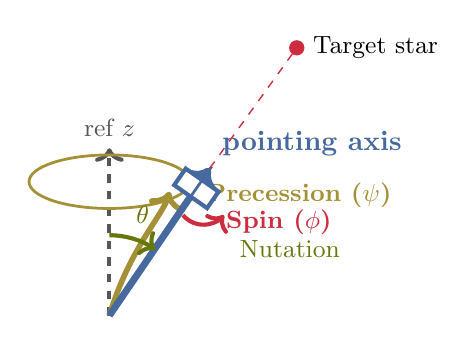
\begin{tikzpicture}[scale=0.85]
    % Reference z-axis
    \draw[->, line width=1.5pt, USC_Black90, dashed] (0,0) -- (0,2.5) node[above] {\small ref $z$};

    % Precession cone
    \draw[USC_Gold, line width=1pt] (0,2) ellipse (1.2 and 0.4);
    \draw[->, line width=2pt, USC_Gold] (0,0) .. controls (0.3,1) and (0.8,1.5) .. (0.9,1.85);
    \node[USC_Gold, font=\bfseries\small, right] at (1.3,1.8) {Precession ($\psi$)};

    % Spacecraft pointing axis (tilted)
    \draw[->, line width=2.5pt, USC_Blue] (0,0) -- (1.5,2.2) node[above right, font=\bfseries] {pointing axis};

    % Nutation angle
    \draw[->, line width=1.5pt, USC_Olive] (0,1.2) arc (90:55:1.2);
    \node[USC_Olive, font=\bfseries\small] at (0.5,1.5) {$\theta$};
    \node[USC_Olive, font=\small, right] at (1.8,1.0) {Nutation};

    % Spin arrow around pointing axis
    \draw[->, line width=1.5pt, USC_Rose] (1.1,1.5) arc (220:320:0.4);
    \node[USC_Rose, font=\bfseries\small, right] at (1.6,1.4) {Spin ($\phi$)};

    % Simple spacecraft shape
    \begin{scope}[shift={(1.3,1.9)}, rotate=55]
        \draw[line width=1.5pt, USC_Blue, fill=white] (-0.15,-0.3) rectangle (0.15,0.3);
        \draw[line width=1pt, USC_Blue] (-0.4,0) -- (0.4,0); % solar panels
    \end{scope}

    % Star target
    \filldraw[USC_Rose] (2.8,4) circle (3pt);
    \node[right, font=\small] at (2.9,4) {Target star};
    \draw[dashed, USC_Rose, line width=0.5pt] (1.5,2.2) -- (2.8,4);
\end{tikzpicture}
\end{document}
